\documentclass{ctexart}
\usepackage{amsmath,bm}
\usepackage{setspace}
\usepackage{xeCJK}
\usepackage{xcolor}
\usepackage{indentfirst}
\usepackage{listings}
\usepackage{graphicx}
\usepackage{subfigure}
\usepackage{amsfonts,amssymb}
\usepackage[a4paper,scale=0.8]{geometry}
\usepackage{hyperref}
\usepackage{float}
\usepackage{listings}
\usepackage{changepage}
\lstset{language=verilog}%这条命令可以让LaTeX排版时将C++键字突出显示

\lstset{breaklines}%这条命令可以让LaTeX自动将长的代码行换行排版

\lstset{extendedchars=false}%这一条命令可以解决代码跨页时,章节标题,页眉等汉字不显示的问题
\setCJKmainfont{华光书宋_CNKI}
\newCJKfontfamily\kaiti{华光楷体_CNKI}
\newCJKfontfamily\hei{华光黑体_CNKI}
\newCJKfontfamily\fsong{华光仿宋_CNKI}
\newfontfamily\code{Courier New}
\linespread{1.5} \setlength\parindent{2 em}
\title{\Huge 中国科学技术大学计算机学院\\《计算机体系结构》实验报告}
\date{\LARGE 2021.05.28}
\begin{document}
\begin{hei}  \maketitle\end{hei}
\begin{figure}[htbp]
    \centering
    
\includegraphics[scale=0.4]{USTC.png}

\end{figure}
\begin{LARGE}\begin{align*} & \text{实验题目:\underline{Cache的设计和实现}} \\
         & \text{学生姓名:\underline{胡毅翔}}            \\
         & \text{学生学号:\underline{PB18000290}}\end{align*}\end{LARGE}
\par
\par\par
\centerline{\large 计算机实验教学中心制}
\par \centerline {\large 2019年9月}
\newpage
\tableofcontents
\newpage
\section{\hei 实验目的}
1.实现组相联度可变的Cache。
\par 2.实现FIFO和LRU替换策略。
\par 3.连接Lab2中实现的CPU并运行测试程序。
\par 4.统计程序运行过程中的miss和hit。
\par 5.权衡cache size增大带来的命中率提升收益和存储资源电路面积的开销。
\par 6.权衡选择合适的组相连度。
\par 7.体会使用复杂电路实现复杂替换策略带来的收益和简单替换策略的优势。
\par 8.理解写回法的优劣。
\section{\hei 实验环境}
1.PC一台\par
2.Windows 10操作系统\par
3.Vivado 2019.1\par
4.Visual Studio Code 1.56.2
\section{\hei Cache设计和实现}
\subsection{\hei Cache结构}
Cache结构在课本《计算机体系结构:量化研究方法》(中文第五版)的附录B:存储器层次结构回顾 中有所描述。本实验全部采用“写回+写入分派”的cache策略,这种策略在读或写命中时,直接从cache中读写数据,只需要一个时钟周期,不需要对CPU流水线进行stall;在发生缺失时,读缺失和写缺失的处理方法是相同的,都是从主存中换入缺失的line(line即块)到cache中(当然,如果要换入的line已经被使用了,并且脏,则需要在换入之前进行换出),再从cache中读写数据。总结下来,cache应该维护如下的状态机:
\begin{figure}[H]
    \centering
    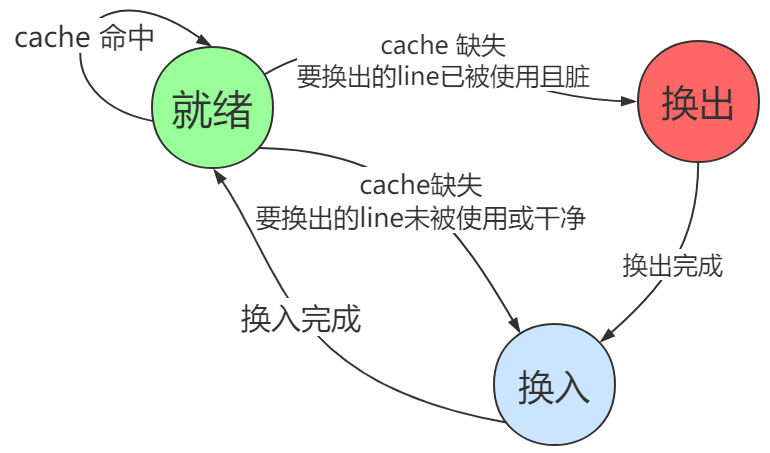
\includegraphics[scale=0.45]{ztj.png}
    \caption{cache状态机}
\end{figure}
\par 当没有读/写请求时,cache保持就绪状态,当CPU发出读/写请求时,cache检查是否命中,如果命中则立刻响应读/写请求,并仍保持就绪状态。如果缺失,则进行换入(换入之前可能需要先换出),在cache进行换出换入时,cache无法响应CPU当前的读写请求,因此需要向CPU发出miss=1的信号,CPU需要使用该信号控制所有流水段进行stall。直到cache完成换出换入后重回就绪状态,此时cache就能响应这个读写请求。
\subsection{\hei Cache对外接口与时序}
cache的对外接口如下:
\begin{lstlisting}
    module cache #(
        parameter LINE_ADDR_LEN = 3,  // line内地址长度,决定了每个line具有2^3个word
        parameter SET_ADDR_LEN = 3,  // 组地址长度,决定了一共有2^3=8组
        parameter TAG_ADDR_LEN = 6,  // tag长度
        parameter WAY_CNT = 4 // 组相连度,决定了每组中有多少路line
    )(
        input clk, rst,
        output miss,  // 对CPU发出的miss信号
        input [31: 0] addr,  // 读写请求地址
        input rd_req,  // 读请求信号
        output reg [31: 0] rd_data,  // 读出的数据,一次读一个word
        input wr_req,  // 写请求信号
        input [31: 0] wr_data // 要写入的数据,一次写一个word
    );
\end{lstlisting}
当读/写命中时,时序与以往的dataRam完全一样,如图:
\begin{figure}[H]
    \begin{minipage}[t]{0.5\linewidth}
        \centering
        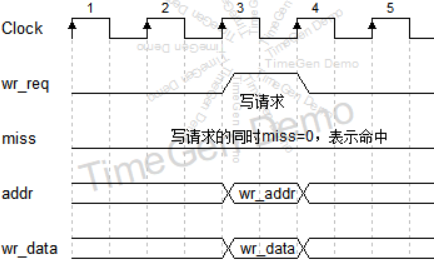
\includegraphics[width=2.2in]{sx1.png}
        \caption{写命中时序}
        \label{fig:side:a}
    \end{minipage}%
    \begin{minipage}[t]{0.5\linewidth}
        \centering
        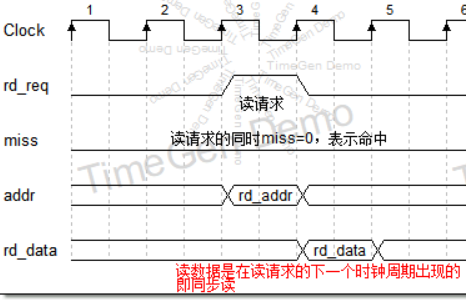
\includegraphics[width=2.2in]{sx2.png}
        \caption{读命中时序}
        \label{fig:side:b}
    \end{minipage}
\end{figure}
\par
当读/写缺失时,随着请求信号的出现,miss信号同样变为1,请
求信号要一直保持1,直到一个周期,miss变为0,请求信号仍为1,就完成了一次读/写。另外,在请求信号保持1的过程中,addr和wr\_data也要保持。
\begin{figure}[H]
    \begin{minipage}[t]{0.5\linewidth}
        \centering
        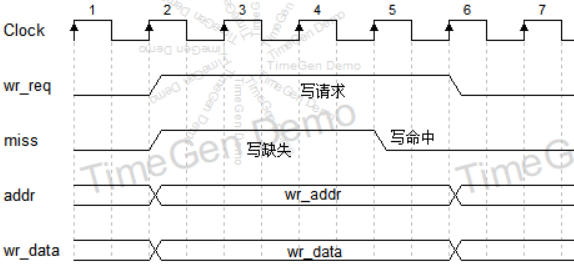
\includegraphics[width=2.2in]{xqs.png}
        \caption{写缺失时序}
        \label{fig:side:a1}
    \end{minipage}%
    \begin{minipage}[t]{0.5\linewidth}
        \centering
        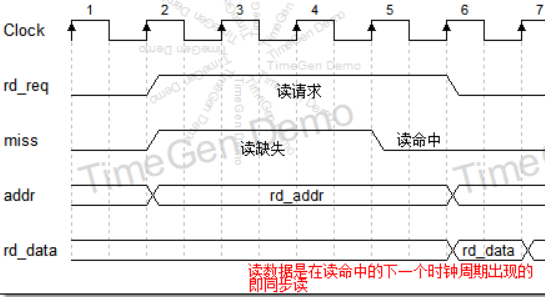
\includegraphics[width=2.2in]{dqs.png}
        \caption{读缺失时序}
        \label{fig:side:b1}
    \end{minipage}
\end{figure}
\par
rd\_req与miss,wr\_req与miss,实际上构成了两对握手信号,这种握手信号时序广泛的应用于总线技术中。
\par 在以上的时序图中,缺失只持续了3个时钟周期,这只是为了方便演示。在本实验中,由于主存需要50个周期进行一次读/写,所以cache缺失会持续50多个时钟周期或100多个时钟周期。当只进行换入时,缺失持续50多个时钟周期。当先换出后换入时,缺失持续100多个时钟周期。
\subsection{\hei 主存对外接口与时序}
主存被cache所调用,是使用BRAM模仿的DDR。包括main\_mem.sv与mem.sv两个文件,顶层文件是main\_mem.sv,它以line为读写单元(而不是以word为读写单元),且读写周期很长,本实验设置为50个时钟周期。
\par main\_mem的输入输出接口定义如下:
\begin{lstlisting}
  module main_mem #(      // 主存,每次读写以line 为单位,并会延时固定的50个周期
  parameter  LINE_ADDR_LEN =  3,  // line内地址的长度,决定了每个line具有2^3=8个word
  parameter  ADDR_LEN  = 8         // 主存一共有2^8=256个line
)(
  input  clk, rst,
  output gnt,                                      // 读写响应信号
  input  [ADDR_LEN-1:0] addr,                     // 读写地址
  input  rd_req,                                   // 读请求信号
  output reg [31:0] rd_line [1<<LINE_ADDR_LEN], // 读出的line数据,这是一个二维数组,即8个word = 8*32bit
  input  wr_req,                                   // 写请求信号
  input  [31:0] wr_line [1<<LINE_ADDR_LEN]        // 要写入的line数据,这是一个二维数组,是8个word = 8*32bit
);

\end{lstlisting}\par
main\_mem的读写时序与cache的读写缺失时序非常相似,也就是说,主存可以看作一个永远都会缺失,并且一缺失就缺失50个周期的cache。不同的是cache的miss信号和main\_mem的gnt信号的逻辑相反:
cache的miss=0时代表命中;而main\_mem的gnt=1时代表命中。如图:\par
\begin{figure}[H]
    \begin{minipage}[t]{0.5\linewidth}
        \centering
        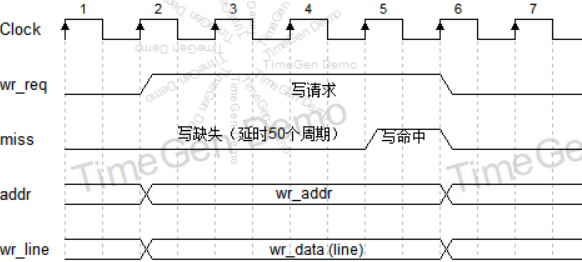
\includegraphics[width=2.2in]{zcx.png}
        \caption{主存写时序}
        \label{fig:side:a2}
    \end{minipage}%
    \begin{minipage}[t]{0.5\linewidth}
        \centering
        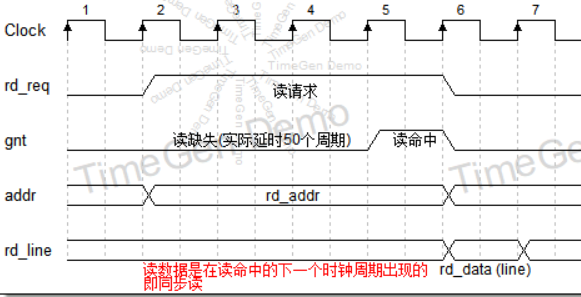
\includegraphics[width=2.2in]{zcd.png}
        \caption{主存读时序}
        \label{fig:side:b2}
    \end{minipage}
\end{figure}
\par
\subsection{\hei 直接映射cache的实现}
理解cache首先要看32bit addr是如何分割的,如下图:\par
\begin{figure}[H]
    \centering
    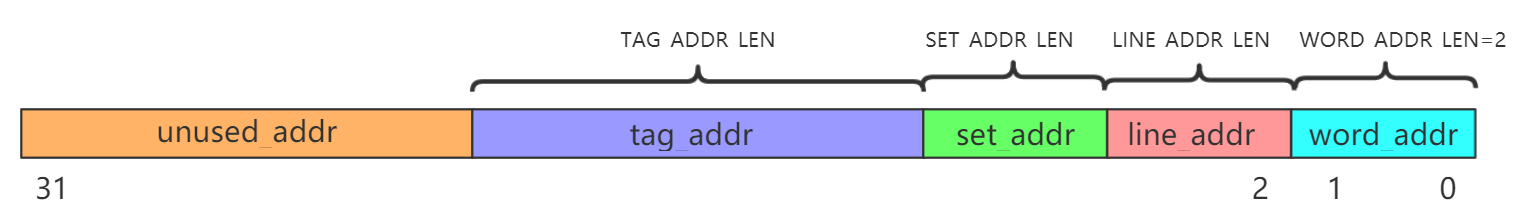
\includegraphics[scale=0.45]{dzfg.png}
    \caption{32bit 地址的分割}
\end{figure}
word\_addr[1:0] :  字节地址,即指定字节是word(字)中的第几个。固定为2bit。本次实验不要求处理独热码,因此word\_addr不需要处理。
\par line\_addr: line内地址,其长度由参数LINE\_ADDR\_LEN决定。例如,如果希望每个line中有16个word,则LINE\_ADDR\_LEN应设为4,因为$2^{4}=16$。在cache读写过程中,line\_addr用于指示要读写的word是line中的哪一个word。
\par set\_addr: line地址,其长度由参数SET\_ADDR\_LEN决定。例如,如果希望cache中有4个cache组,则SET\_ADDR\_LEN应该设置为2,因为$2^{2}=4$。在cache读写过程中,set\_addr负责将读写请求路由到正确的组。
\par tag\_addr: 是该32位地址的TAG。当发生读写请求时,cache应该把32位地址中的tag\_addr取出,与cache中的TAG比较,如果相等则命中。如果不等则缺失。
\par unused\_addr: 32位地址中的高位,直接丢弃。
\par 在我们提供的代码中,使用一句assign完成32bit地址的分割:
\begin{lstlisting}
assign {unused_addr, tag_addr, set_addr, line_addr, word_addr} = addr;
\end{lstlisting}\par
在简单cache中,line\space size可以通过调节LINE\_ADDR\_LEN去改变,组数可以通过调节SET\_ADDR\_LEN去改变。这里,以LINE\_ADDR\_LEN=3,SET\_ADDR\_LEN=2, TAG\_ADDR=12为例,给出直接相连cache的结构图:
\begin{figure}[H]
    \centering
    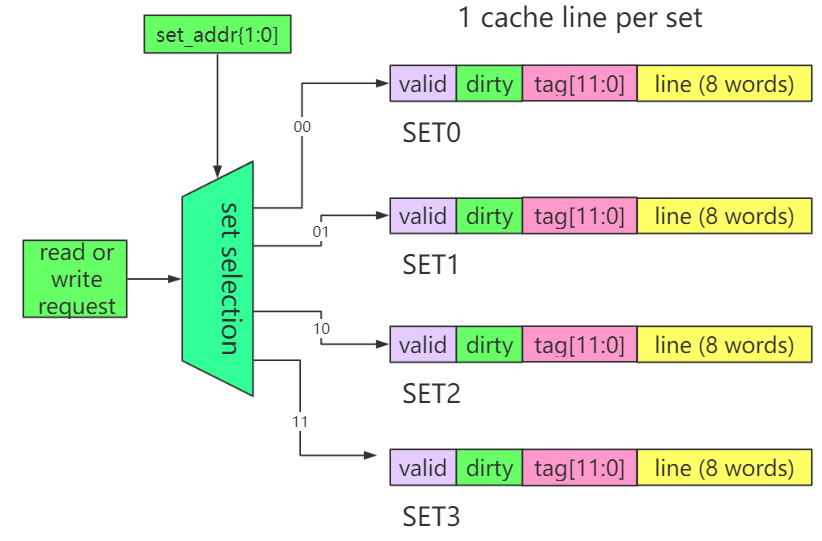
\includegraphics[scale=0.55]{zjxl.png}
    \caption{直接相连cache的结构}
\end{figure}
\par 实际上,直接相连是组相连的特殊情况,相当于1路组相连,因此每个set中只有1个line。每个 line是8个word,除此之外,每个line还需要1个TAG,一个dirty(脏位),一个valid(有效位)。这些在system\space verilog代码里如下:
\par \begin{figure}[H]
    \centering
    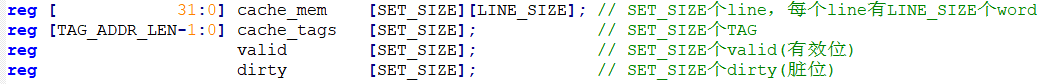
\includegraphics[scale=0.65]{zjxlbl.png}
    \caption{直接相连cache中的一些变量}
\end{figure}
\par 当有读写请求时,根据地址中的set\_addr字段,决定要到哪个line中读写数据。然后,查看该line是否valid,如果valid=0则一定是缺失,如果valid=1,说明这个line是有效的,需要比较这个line的tag和地址中的tag是否相同,相同则命中,不同则缺失。如果命中,则立即响应读写请求。当然,如果是写请求,要把dirty置1。
\par 如果cache缺失,要从主存中换入该块到这个cache line中。在换入前,也需要考虑是否需要先换出。如果valid=1且dirty=1,说明该cache块是有效的并且已经被修改过,则需要先进行换出。此时需要控制cache状态机的状态转移。cache状态机的状态如下:
\begin{lstlisting}
    enum  {IDLE, SWAP_OUT, SWAP_IN, SWAP_IN_OK} cache_stat = IDLE;
    \end{lstlisting}
\par 相比图1,这里多出一个状态SWAP\_IN\_OK,该状态一定出现在SWAP\_IN状态之后,只占用一个时钟周期,负责把主存中读出的数据写入cache\space line。
\subsection{\hei 组相连cache的实现}
下图是组相连cache的结构图。取LINE\_ADDR\_LEN=3,SET\_ADDR\_LEN=2, TAG\_ADDR=12,WAY\_CNT=4为例。
\par
\par \begin{figure}[H]
    \centering
    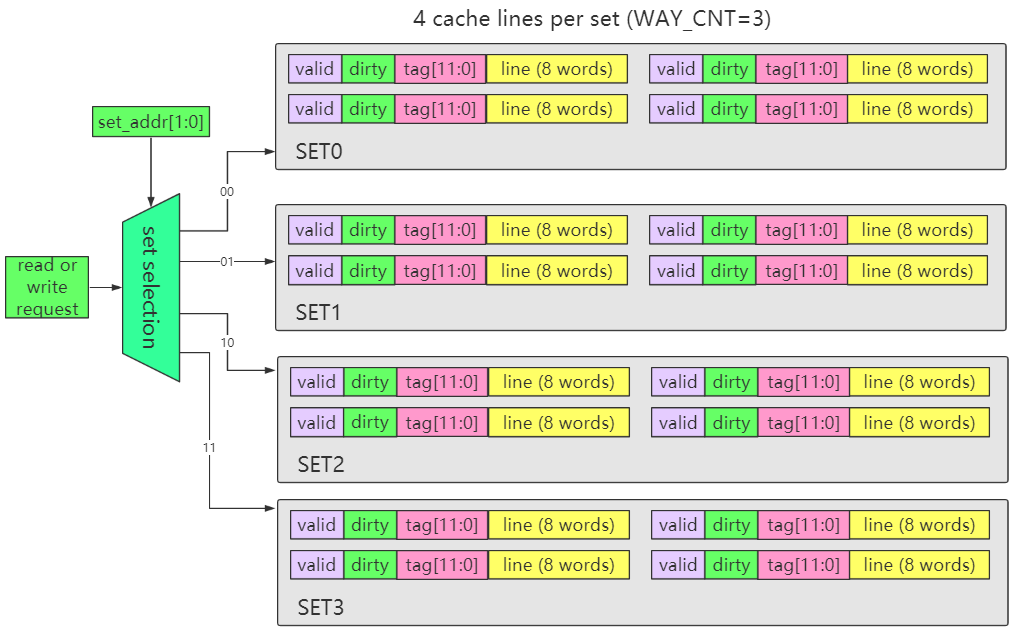
\includegraphics[scale=0.65]{4lzxl.png}
    \caption{4路组相连cache}
\end{figure}
\par 相比直接相连cache,组相连cache需要加入的有:
\begin{enumerate}
    \item 将图10中所示的数组添加一个维度,该维度的大小为 WAY\_CNT。
    \item 实现并行命中判断:为了判断是否命中,直接相连cache每次只需要判断一个valid,一个dirty,一个TAG是否命中,但组相连cache则需要在组内并行的判断每路line是否命中。
    \item 实现替换策略:当cache需要换出时,直接相连cache没有选择,因为每个组中只有1个line,只能换出换入这唯一的line。但组相连cache需要决策换出哪个line。本实验要求实现FIFO换出策略与LRU换出策略(请见《计算机体系结构:量化研究方法》(中文第五版)附录B)。为了实现FIFO策略和LRU策略,还需要加入一些辅助的wire和reg变量。
\end{enumerate}
\section{\hei 替换策略的实现}
\subsection{\hei FIFO}
FIFO(First\space In\space First\space Out)算法,即先入先出,替换规则为将最早存入的块换出。在代码中,增加如下数据结构:
\begin{lstlisting}
    reg [WAY_CNT: 0] FIFO_record[SET_SIZE][WAY_CNT]; //每一组内的FIFO排位记录
\end{lstlisting}
\par 每次存入新块时,更新FIFO\_record,替换时的算法为:
\begin{lstlisting}
begin
    for (integer i = 0;i < WAY_CNT ;i = i + 1)
    begin //此时说明是最早进去的
        if (FIFO_record[set_addr][i] == WAY_CNT)
        begin
            out_way = i;
            FIFO_record[set_addr][i] = 0;
            break;
        end
    end
end
\end{lstlisting}
\subsection{\hei LRU}
LRU(Least\space Recent\space Use)算法,即最近最少使用,替换规则为将最近使用时间最早的块换出。在代码中,增加如下数据结构:
\begin{lstlisting}
integer time_cnt; //LRU时间记录
reg [15: 0] LRU_record[SET_SIZE][WAY_CNT]; //每一项的LRU记录
\end{lstlisting}
\par 每个时钟周期更新time\_cnt,使用块时,更新LRU\_record。选择换出的块时使用以下算法:
\begin{lstlisting}
if (swap_out_strategy == LRU)
begin
    for (integer i = 0; i < WAY_CNT; i = i + 1 )
    begin
        out_way = 0;
        if (LRU_record[set_addr][i] < LRU_record[set_addr][out_way])
        begin
            out_way = i;
        end
    end
end
\end{lstlisting}
\section{\hei Cache资源消耗评估}

在cache.sv中修改Cache的参数(组数、组相连度、line大小等),进行综合得到资源占用报告。其中LUT、FF是我们最在意的资源,因为cache的逻辑均使用LUT和FF实现。
这两个参数的使用量就代表了cache所占用电路的资源量。
多次修改参数得到下表:
\begin{table}[H]
    \centering
    \begin{tabular}{ccccc}
        \textbf{组数} & \textbf{组相联度} & \textbf{line size} & \textbf{LUT} & \textbf{FF} \\
        8             & 4                 & 8                  & 1128         & 3056        \\
        8             & 2                 & 8                  & 1131         & 3057        \\
        8             & 1                 & 8                  & 1141         & 3057        \\
        4             & 4                 & 8                  & 1997         & 3210        \\
        16            & 4                 & 8                  & 4075         & 9912        \\
        8             & 4                 & 4                  & 1532         & 3030        \\
        8             & 4                 & 16                 & 4138         & 10295
    \end{tabular}
    \caption{不同Cache的资源占用情况}
\end{table}
\par 根据表中数据,我们可以得出以下结论:
\begin{enumerate}
    \item 修改组相联度对cache所占资源数变化不大。
    \item 增加组数或增大line\space size都会增加资源消耗。
\end{enumerate}
\section{\hei Cache与CPU组合测试}
设置组数为8,组相联度为4,每个line内有8个word,分别测试在规模为256的快速排序,规模为$16\times 16$矩阵乘法上对FIFO,LRU两种替换策略进行测试。
\begin{table}[H]
    \centering
    \begin{tabular}{cccccc}
        \textbf{替换策略} & \textbf{测试样例} & \textbf{组相联度} & \textbf{miss} & \textbf{hit} & \textbf{命中率} \\
        FIFO              & 矩阵乘法          & 4                 & 4800          & 3904         & 44.85\%         \\
        LRU               & 矩阵乘法          & 4                 & 4696          & 4008         & 46.04\%         \\
        LRU               & 矩阵乘法          & 8                 & 4696          & 4008         & 46.04\%         \\
        FIFO              & 快速排序          & 4                 & 142           & 5322         & 97.40\%         \\
        LRU               & 快速排序          & 4                 & 247           & 5217         & 95.48\%         \\
        LRU               & 快速排序          & 1                 & 247           & 5217         & 95.48\%         \\
        LRU               & 快速排序          & 2                 & 247           & 5217         & 95.48\%         \\
        LRU               & 快速排序          & 8                 & 247           & 5217         & 95.48\%
    \end{tabular}
    \caption{不同替换策略的缓存命中情况}
    \par 根据表中数据,我们可以得出以下结论:
    \begin{enumerate}
        \item LRU和FIFO在测试程序中的表现差异不大。
        \item FIFO算法虽然更为简单,但在快速排序中有着更好的效果。
    \end{enumerate}
\end{table}
\section{\hei 总结}
本次实验完成了组相联Cache的设计,实现了FIFO和LRU两种替换策略,并与CPU连接,运行测试程序。通过数据实验加深了对课程内容的理解。
\end{document}